\subsection{Phân hệ Quản trị Nhân sự (HRM Module)}
\label{subsec:module_hrm}

\subsubsection{Mô tả Nghiệp vụ và Yêu cầu Chức năng}
Phân hệ Quản trị Nhân sự là một trong hai trụ cột nghiệp vụ lớn nhất của ứng dụng di động MyHCMUT, kết nối trực tiếp với dịch vụ nghiệp vụ nhân sự \texttt{hrm-be} và cơ sở dữ liệu \texttt{tcns-dev} của Nhà trường:

\begin{itemize}
    \item \textbf{Quản lý Hồ sơ Lý lịch 11 Danh mục:} Tra cứu toàn diện thông tin cá nhân, đào tạo, ngạch bậc lương, hợp đồng, khen thưởng, kỷ luật, quá trình công tác...; hỗ trợ lưu đệm ngoại tuyến qua SQLite.
    \item \textbf{Đề xuất \& Thẩm định Sửa Lý lịch (Diff Viewer):} Cán bộ gửi đề xuất cập nhật kèm ảnh minh chứng; Chuyên viên Phòng TCCB thẩm định qua giao diện so sánh trực quan sai khác giữa giá trị cũ và giá trị mới trước khi duyệt ghi đè vào hồ sơ chính thức.
    \item \textbf{Đăng ký Nghỉ phép Wizard 4 bước:} Thiết kế Form Wizard 4 bước kết hợp thuật toán kiểm tra ràng buộc thời gian thực 4 tầng từ API \texttt{POST /api/tcns-nghi-phep/validate}:
    \begin{enumerate}
        \item Tính toán chính xác số ngày làm việc thực tế (tự động loại trừ Thứ 7, Chủ nhật và ngày Lễ theo quy định).
        \item Kiểm tra phát hiện trùng lặp lịch nghỉ phép hoặc lịch công tác cá nhân.
        \item Kiểm tra mốc nộp trễ hạn (cảnh báo bắt buộc nhập lý do giải trình nếu nộp trễ quá 3 ngày hoặc 15 ngày tùy loại phép).
        \item Kiểm tra đối soát số dư quỹ phép năm trong bảng \texttt{tcns\_so\_nghi\_phep\_nam}.
    \end{enumerate}
    \item \textbf{Đăng ký \& Phê duyệt Đi công tác (Business Trip):} Cán bộ lập kế hoạch chuyến đi, chọn thành viên đoàn công tác, nhập địa điểm, thời gian, dự toán kinh phí và đính kèm thư mời/kế hoạch PDF; Lãnh đạo Đơn vị và BGH thẩm định phê duyệt đa cấp.
    \item \textbf{Phê duyệt Đơn Hàng loạt (\texttt{AppBatchActionBar}):} Cho phép Lãnh đạo Đơn vị chọn nhiều đơn nghỉ phép hoặc công tác cùng lúc để duyệt hàng loạt chỉ bằng một thao tác, tối ưu hóa thời gian xử lý hành chính.
\end{itemize}

\subsubsection{Đặc tả Ca sử dụng (Use Cases)}

\begin{table}[H]
\centering
\renewcommand{\arraystretch}{1.2}
\small
\begin{tabularx}{\textwidth}{|L{3.2cm}|Y|}
\hline
\textbf{Mã Ca sử dụng} & \textbf{UC\_HRM\_01: Tra cứu \& Thẩm định Chỉnh sửa Lý lịch Cán bộ (Diff Viewer)} \\
\hline
\textbf{Tác nhân} & Cán bộ / Giảng viên (Người gửi), Chuyên viên Phòng TCCB (Người duyệt) \\
\hline
\textbf{Tiền điều kiện} & Cán bộ đã đăng nhập thành công vào ứng dụng MyHCMUT. \\
\hline
\textbf{Hậu điều kiện} & Dữ liệu hồ sơ lý lịch được cập nhật chính thức vào cơ sở dữ liệu nhân sự của Nhà trường. \\
\hline
\textbf{Luồng sự kiện chính} & 
1. Cán bộ mở màn hình \texttt{PersonalProfilePage}, xem 11 danh mục lý lịch chi tiết. \newline
2. Cán bộ chọn trường thông tin cần chỉnh sửa, nhập giá trị mới và đính kèm tệp ảnh minh chứng. \newline
3. Nhấn \textit{``Gửi đề xuất''} $\rightarrow$ Hệ thống ghi nhận vào bảng \texttt{staff\_ly\_lich\_request} ở trạng thái \texttt{PENDING} và phát sự kiện thông báo cho Phòng TCCB. \newline
4. Chuyên viên TCCB mở màn hình \texttt{ApproveProfileDetailPage}, xem thẻ \texttt{ReviewDiffCard} đối chiếu trực quan giá trị cũ (màu đỏ) và giá trị mới (màu xanh lá). \newline
5. Chuyên viên nhấn \textit{``Phê duyệt''} $\rightarrow$ Hệ thống cập nhật dữ liệu mới vào \texttt{staff\_ly\_lich} và gửi thông báo hoàn tất cho Cán bộ. \\
\hline
\textbf{Luồng ngoại lệ} & Nếu Chuyên viên chọn \textit{``Từ chối''}, bắt buộc nhập lý do từ chối $\rightarrow$ Bản ghi chuyển trạng thái \texttt{REJECTED} và thông báo cho Cán bộ biết. \\
\hline
\end{tabularx}
\caption{\textit{Đặc tả Ca sử dụng UC\_HRM\_01: Tra cứu và Thẩm định Sửa Lý lịch}}
\label{tab:uc_hrm_01}
\end{table}

\begin{table}[H]
\centering
\renewcommand{\arraystretch}{1.2}
\small
\begin{tabularx}{\textwidth}{|L{3.2cm}|Y|}
\hline
\textbf{Mã Ca sử dụng} & \textbf{UC\_HRM\_02: Đăng ký Nghỉ phép Form Wizard 4 bước \& Validate Thời gian thực} \\
\hline
\textbf{Tác nhân} & Cán bộ / Giảng viên \\
\hline
\textbf{Tiền điều kiện} & Cán bộ đã đăng nhập; còn tài khoản hoạt động trong hệ thống. \\
\hline
\textbf{Hậu điều kiện} & Đơn nghỉ phép được khởi tạo thành công ở trạng thái \texttt{CHO\_DUYET} và kích hoạt quy trình phê duyệt. \\
\hline
\textbf{Luồng sự kiện chính} & 
1. Cán bộ mở màn hình \texttt{LeaveRequestPage}, bắt đầu Bước 1: Chọn loại nghỉ và lý do nghỉ. \newline
2. Bước 2: Chọn khoảng thời gian (Từ ngày $\rightarrow$ Đến ngày). \newline
3. Hệ thống tự động gọi API \texttt{POST /api/tcns-nghi-phep/validate} để thực thi 4 tầng kiểm tra: (a) Tính số ngày làm việc thực tế, (b) Kiểm tra trùng lịch cá nhân, (c) Kiểm tra mốc nộp trễ hạn, (d) Kiểm tra số dư quỹ phép năm. \newline
4. Nếu vi phạm mốc nộp trễ hạn $\rightarrow$ Bước 3 hiển thị trường bắt buộc nhập lý do giải trình nộp trễ. \newline
5. Bước 4: Cán bộ xác nhận cam kết bàn giao công việc và nhấn nút \textit{``Gửi duyệt''}. \newline
6. Hệ thống lưu bản ghi vào \texttt{tcns\_nghi\_phep\_dang\_ky} và đẩy thông báo tới Lãnh đạo Đơn vị. \\
\hline
\textbf{Luồng ngoại lệ} & Nếu số ngày nghỉ vượt quá số ngày phép còn lại hoặc trùng với lịch công tác đã duyệt $\rightarrow$ Hệ thống cảnh báo đỏ và khóa không cho phép chuyển bước. \\
\hline
\end{tabularx}
\caption{\textit{Đặc tả Ca sử dụng UC\_HRM\_02: Đăng ký Nghỉ phép 4 bước}}
\label{tab:uc_hrm_02}
\end{table}

\begin{table}[H]
\centering
\renewcommand{\arraystretch}{1.2}
\small
\begin{tabularx}{\textwidth}{|L{3.2cm}|Y|}
\hline
\textbf{Mã Ca sử dụng} & \textbf{UC\_HRM\_03: Đăng ký \& Phê duyệt Đi công tác (Business Trip)} \\
\hline
\textbf{Tác nhân} & Cán bộ đăng ký, Lãnh đạo Đơn vị, Ban Giám hiệu / Phòng TCCB \\
\hline
\textbf{Tiền điều kiện} & Cán bộ có kế hoạch đi công tác trong hoặc ngoài nước. \\
\hline
\textbf{Hậu điều kiện} & Chuyến đi công tác được phê duyệt chính thức và cập nhật vào lịch trình công tác. \\
\hline
\textbf{Luồng sự kiện chính} & 
1. Cán bộ mở màn hình \texttt{BusinessTripEditPage}, nhập mục đích, địa điểm, thời gian, phương tiện di chuyển, dự toán kinh phí và chọn danh sách thành viên đoàn. \newline
2. Đính kèm tệp tài liệu PDF (thư mời, kế hoạch công tác) $\rightarrow$ Nhấn \textit{``Gửi duyệt''}. \newline
3. Lãnh đạo Đơn vị nhận thông báo đẩy FCM, mở \texttt{ApproveBtripListPage} xem xét nội dung $\rightarrow$ Nhấn \textit{``Phê duyệt''}. \newline
4. Nếu chuyến công tác yêu cầu cấp trường phê duyệt $\rightarrow$ Hệ thống chuyển tiếp lên Ban Giám hiệu / Phòng TCCB duyệt và cấp số quyết định. \newline
5. Hệ thống chuyển trạng thái \texttt{DA\_DUYET} và thông báo tới toàn bộ thành viên đoàn công tác. \\
\hline
\end{tabularx}
\caption{\textit{Đặc tả Ca sử dụng UC\_HRM\_03: Đăng ký và Phê duyệt Đi công tác}}
\label{tab:uc_hrm_03}
\end{table}

\subsubsection{Biểu đồ Hoạt động (Activity Diagrams)}

\begin{figure}[H]
    \centering
    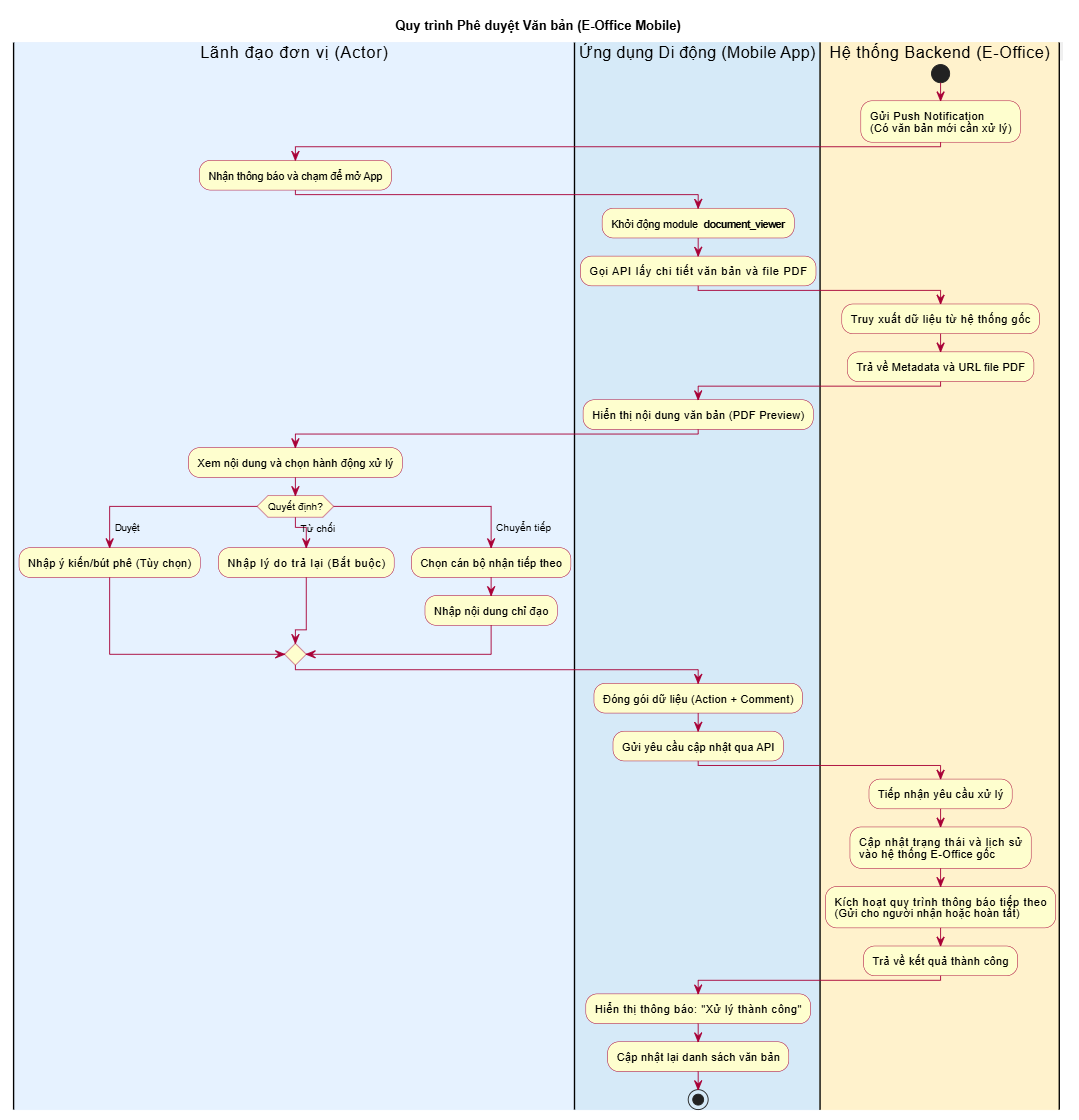
\includegraphics[width=0.85\linewidth]{img/uml/activity_leave_process.png}
    \caption{\textit{Biểu đồ Hoạt động Quy trình Đăng ký và Phê duyệt Nghỉ phép}}
    \label{fig:act_hrm_leave}
\end{figure}

\begin{figure}[H]
    \centering
    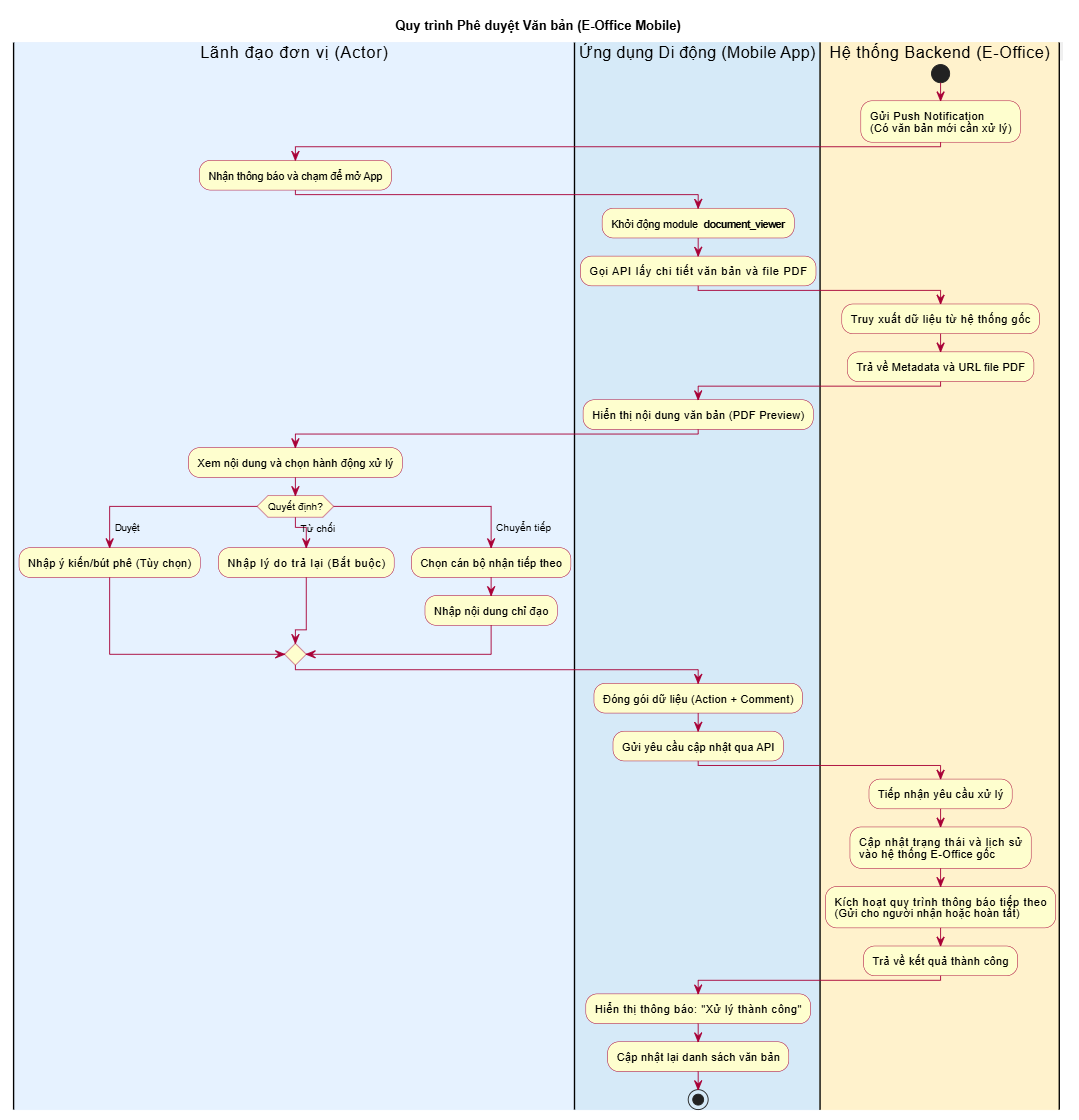
\includegraphics[width=0.85\linewidth]{img/uml/activity_business_trip.png}
    \caption{\textit{Biểu đồ Hoạt động Quy trình Đăng ký và Phê duyệt Đi công tác}}
    \label{fig:act_hrm_btrip}
\end{figure}

\subsubsection{Biểu đồ Tuần tự (Sequence Diagrams)}

\begin{figure}[H]
    \centering
    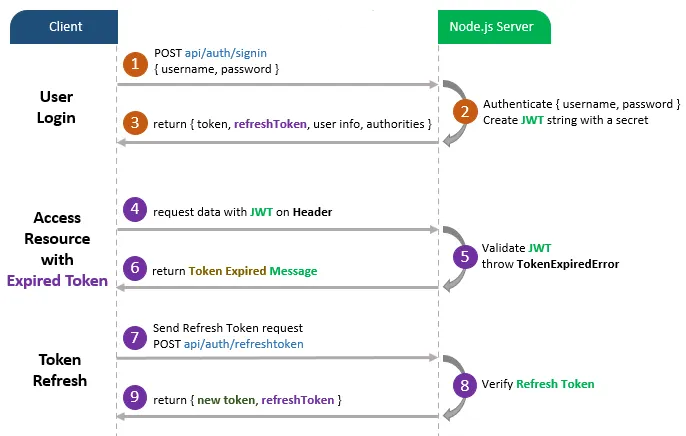
\includegraphics[width=0.85\linewidth]{img/uml/seq_leave_validation.png}
    \caption{\textit{Biểu đồ Tuần tự Đăng ký và Kiểm tra Ràng buộc Nghỉ phép Thời gian thực}}
    \label{fig:seq_hrm_leave_val}
\end{figure}

\begin{figure}[H]
    \centering
    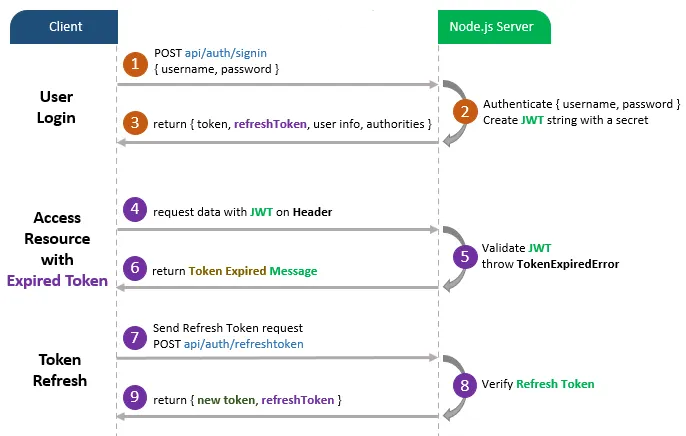
\includegraphics[width=0.85\linewidth]{img/uml/seq_leave_approval.png}
    \caption{\textit{Biểu đồ Tuần tự Phê duyệt Đơn Nghỉ phép Đa cấp}}
    \label{fig:seq_hrm_leave_app}
\end{figure}

\begin{figure}[H]
    \centering
    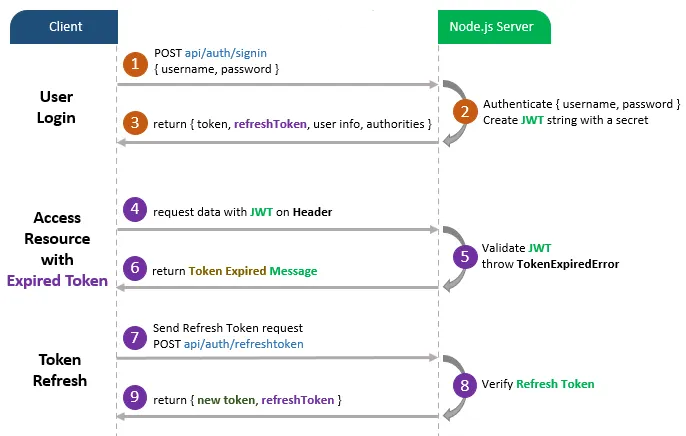
\includegraphics[width=0.85\linewidth]{img/uml/seq_business_trip.png}
    \caption{\textit{Biểu đồ Tuần tự Đăng ký và Phê duyệt Chuyến Đi công tác}}
    \label{fig:seq_hrm_btrip}
\end{figure}

\begin{figure}[H]
    \centering
    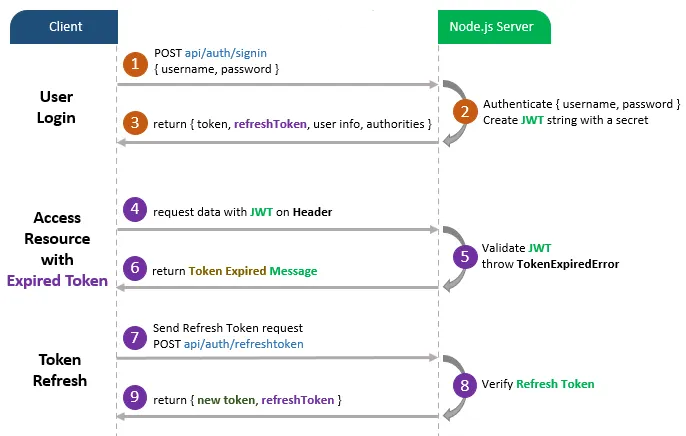
\includegraphics[width=0.85\linewidth]{img/uml/seq_profile_diff.png}
    \caption{\textit{Biểu đồ Tuần tự Thẩm định So sánh Sai khác (Diff Viewer) Sửa Lý lịch}}
    \label{fig:seq_hrm_diff}
\end{figure}
